% INFO6003 Final Report -- Version 11: v10 plus the 30 Oct re-runs (byte-identical reproduction, trunk refit of 1439, point-resampling sensitivity).
% Compile: pdflatex twice (class llncs.cls, figures/ folder). Bibliography embedded.
\documentclass[runningheads]{llncs}
\usepackage[T1]{fontenc}
\usepackage[utf8]{inputenc}
\usepackage{amsmath}
\usepackage{newtxtext}
\usepackage[varvw]{newtxmath}
\usepackage{graphicx}
\usepackage{booktabs,array}
\usepackage{tikz}
\usetikzlibrary{positioning,arrows.meta}
\usepackage{xurl}
\usepackage[hidelinks]{hyperref}
\usepackage{microtype}
\urlstyle{tt}

% Placeholder highlighting: set \highlighttrue for review copies, \highlightfalse for submission.
\usepackage{xcolor}
\usepackage{soulutf8}
\newif\ifhighlight \highlightfalse
\sethlcolor{yellow}
\soulregister{\cite}{7}\soulregister{\ref}{7}\soulregister{\texttt}{1}
\ifhighlight
  \newcommand{\todo}[1]{{\bfseries\hl{[To be completed: #1]}}}
  \newcommand{\pend}{{\bfseries\hl{[pending]}}}
  \newcommand{\verify}{{\bfseries\hl{[VERIFY]}}}
  \newcommand{\figplaceholder}[2]{\fcolorbox{black}{yellow}{\parbox[c][#1][c]{0.95\linewidth}{\centering\small\textbf{Figure placeholder.} #2}}}
\else
  \newcommand{\todo}[1]{\textbf{[To be completed: #1]}}
  \newcommand{\pend}{\textbf{[pending]}}
  \newcommand{\verify}{\textbf{[VERIFY]}}
  \newcommand{\figplaceholder}[2]{\fbox{\parbox[c][#1][c]{0.95\linewidth}{\centering\small\textbf{Figure placeholder.} #2}}}
\fi
\newcolumntype{L}[1]{>{\raggedright\arraybackslash}p{#1}}

\begin{document}
\title{Semi-Automated Individual-Tree Segmentation of Blue Mountains TLS Point Clouds: From Automated Extraction and Manual Refinement to Tree Measurements}
\titlerunning{Semi-Automated Individual-Tree Segmentation of Blue Mountains TLS Data}
\author{Hoang Truong Thinh Nguyen (Thomas) (student ID: 22083142)}
\authorrunning{\mbox{}}
\institute{School of Computer, Data and Mathematical Sciences,\\Western Sydney University}
\maketitle

\begin{abstract}
Measuring single trees in terrestrial laser scanning (TLS) requires each point to be assigned to its tree, which automated methods struggle with where eucalypt crowns overlap. I applied a semi-automated workflow to a 1\,cm TLS scan of Blue Mountains plot WSF\_ML2A. I cut a 57.3\,m $\times$ 55.0\,m area (0.32\,ha) and reduced it to 3\,cm point spacing (45.4 million points). RayCloudTools split it automatically into 162 trees, and two rounds of manual correction in CloudCompare gave 163 tree point clouds. Of these, 86 are identical to an automated tree, and the overlap score ($F_1$ at IoU~$\geq$~0.5) is 0.85. I measured height, stem diameter at breast height (DBH) and crown size for all 163 trees with the ITSMe package, and labelled every value VALID, REVIEW (use with care) or not available. Heights exist for all trees (73 VALID, median 15.6\,m). DBH was measured for 86 trees (42 VALID, median 26.8\,cm), and 40 more have a labelled estimate. Only 16 trees have all four main values VALID: successful segmentation does not guarantee usable measurements, and near-equal tree counts before and after correction hid substantial splitting and merging. I located the georeferenced 30\,m field inventory plot (26 live trees) inside the TLS crop. Within it, the measured TLS DBH has a median of 28--30\,cm against 32.5\,cm in the field, with no significant difference between the distributions. Using two hand-picked anchor trees and the site map, 5 tagged trees were matched with confidence (far more than chance), and their TLS DBH agrees with the field within a few centimetres; several of the largest trees were missed or underestimated because of oval or merged trunks. Height has no field reference.
\keywords{Terrestrial laser scanning \and Individual-tree segmentation \and Manual refinement \and ITSMe \and Measurement quality}
\end{abstract}

%======================================================================
\section{Introduction}\label{sec:intro}

\subsubsection{Motivation.}
Conventional forest inventories record species and stem diameter at breast height (DBH), whereas TLS captures the surfaces of stems, branches and crowns, enabling measurements such as branch architecture and woody volume that are impractical in the field~\cite{calders2020}. These tree-level products require each point to be assigned to one tree. Errors propagate: a merged crown inflates the attributes of one tree and removes those of another, and an omitted stem reduces completeness~\cite{calders2020,cherlet2026}. Segmentation remains the most challenging step to automate, and manual quality control is still needed, particularly in dense forests~\cite{cherlet2026,cushman2026}. For the Blue Mountains monitoring network, the project team identified overlapping eucalypt crowns and complex branching as the main obstacles to automation, and agreed a semi-automated approach: automated extraction followed by manual correction~\cite{meetingnotes,pipeline}. My project applies, documents and measures the output of this approach.

\subsubsection{Research Questions and Objectives.}
The agreed minimum scope is one well-segmented plot, or a large part of one, with biomass analysis and documentation~\cite{meetingnotes}. I ask four questions:
\begin{itemize}
\item[\textbf{RQ1}] What mistakes does automatic segmentation (Rayextract) make in the chosen area, and what does manual correction change?
\item[\textbf{RQ2}] How much manual effort does the correction need?
\item[\textbf{RQ3}] For how many corrected trees can height, DBH and crown size be measured to predefined quality criteria, and why do the others fail?
\item[\textbf{RQ4}] How does TLS DBH, the only trait measured in the field, compare with the field inventory inside the 30\,m field plot?
\end{itemize}
Biomass was part of the agreed scope. Reliable biomass estimates need robust individual-tree segmentation and structural measurements, and the results below show clear limits at exactly these earlier stages. I therefore treat biomass as a later step.

\subsubsection{Contribution.}
I used existing tools and did not develop their methods~\cite{lowe2021,terryn2023}. My supervisor suggested the overall workflow~\cite{pipeline}. Applying it to WSF\_ML2A, correcting the segmentation and measuring the trees is my own work (with the AI help declared at the end). My contributions are: (C1) a 163-tree dataset made by automatic segmentation and two rounds of manual correction; (C2) height, DBH and crown measurements for every tree, each with a quality label; and (C3) a DBH comparison with the field inventory inside the located 30\,m field plot, and a tree-by-tree match of tagged trees to TLS stems. Erick Calderon-Morales and I accepted all 163 trees as the final set, as further correction could not improve them.

%======================================================================
\section{Related Work}\label{sec:related}

\subsubsection{From Point Clouds to Tree-Level Measurements.}
Calders et al.~\cite{calders2020} describe TLS processing as a chain of registration, tree extraction and modelling. Most extraction methods grow detected stems upwards into crowns and need manual correction of missed and wrongly added trees, more so where crowns touch.

\subsubsection{Automated Segmentation and Its Limits.}
Cherlet et al.~\cite{cherlet2026} compare five methods (Rayextract, Treeiso, SSSC, TreeLearn and ForAINet) on 2,983 manually segmented trees in four forest types. The graph-based Rayextract, used here, had the highest plot-level $F_1$ score on three of the four plots (0.480--0.919 across plots), but every method did worse in the dense tropical plot, and accuracy fell with distance from the tree centre. Methods with similar scores made different errors, so the authors expect manual checking to remain part of semi-automated workflows~\cite{cherlet2026}.

\subsubsection{Manual Segmentation and Measurement Quality.}
Manual segmentation is the most accurate method but slow, and operator bias remains in complex areas~\cite{cherlet2026}; Cushman et al.~\cite{cushman2026} call it a bottleneck. They also note that DBH is usually fitted to a thin slice of the stem and gets worse with few points or hidden stems, that ground-based TLS can underestimate height because treetops are sparsely scanned, and that field measurements are themselves uncertain. ITSMe provides such single-tree measurements~\cite{terryn2023}. No benchmark plot is a temperate eucalypt forest~\cite{cherlet2026}. This project therefore documents a complete semi-automated workflow on Blue Mountains data and reports how many trees give measurements that meet predefined quality criteria.

%======================================================================
\section{Data}\label{sec:data}

\subsection{TLS Scan and Study Area}\label{sec:tls}
The meeting notes describe 36 monitoring plots in dry sclerophyll forest, wet sclerophyll forest and rainforest~\cite{meetingnotes}. I did not collect the scans. I used plot WSF\_ML2A, scanned on 12 May 2025 at 1\,cm resolution. The raw scan has 355,462,232 points. From it I cut two areas (``35x35'' and ``55x55''), but only the ``55x55'' area at 3\,cm spacing was corrected and measured. This area is a rectangle of 57.3\,m $\times$ 55.0\,m (0.32\,ha), tilted about 13\textdegree{} to the map axes; I calculated its shape from the points because no boundary file was supplied. In this report, \emph{TLS crop} always means this 0.32\,ha area. The points are georeferenced in WGS~84 / UTM zone 56S (EPSG:32756). The scanner model and scan positions were not supplied.

\subsection{Field Inventory Plot}\label{sec:field}
My professor supplied the field inventory \texttt{TreeData.csv}~\cite{treedata}, and my supervisor later supplied the plot metadata~\cite{plotdata} and a site map~\cite{sitemap}. The \emph{field plot} is a circle of 30\,m diameter (0.071\,ha, about a fifth of the TLS crop), surveyed on 3 April 2024, 13 months before the scan. Its centre and its north, east, south and west posts have GDA94 latitude and longitude. The inventory has 29 records for WSF\_ML2A; 26 are live trees with a DBH of at least 11.2\,cm, listed by quadrant (NE, SE, NW, SW) with species and tag number (1430--1455). DBH is in centimetres (site map legend). There are no tree coordinates and no tree heights; the site description gives a canopy height of 15--25\,m. The site map draws the tagged trees to scale with a north arrow, but its positions are approximate and not georeferenced. 

%======================================================================
\section{Methods}\label{sec:method}

\subsection{Workflow Overview}
My supervisor's steps~\cite{pipeline} end with manual correction. I added a check of which points belong to which tree, quality-labelled measurements, and a before/after comparison. Figure~\ref{fig:pipeline} and Table~\ref{tab:stages} show the five stages.

\begin{figure}[!tb]
\centering
\begin{tikzpicture}[font=\scriptsize, node distance=3mm and 3.2mm,
  box/.style={draw, rounded corners=2pt, align=center, minimum height=9mm, text width=17.5mm, inner sep=2pt},
  done/.style={box, very thick},
  prog/.style={box, very thick, fill=black!10},
  plan/.style={box, dashed},
  arr/.style={-{Latex[length=1.6mm]}}]
\node[done] (s1) {S1 Data\\preparation};
\node[done, right=of s1] (s2) {S2 Automatic\\segmentation};
\node[done, right=of s2] (s3) {S3 Manual\\correction};
\node[done, right=of s3] (s4) {S4 Tree\\measurements};
\node[prog, right=of s4] (s5) {S5 Field\\comparison};
\node[done, below=5mm of s3] (ba) {Before/after\\comparison};
\draw[arr] (s1)--(s2); \draw[arr] (s2)--(s3); \draw[arr] (s3)--(s4); \draw[arr] (s4)--(s5);
\draw[arr] (s3)--(ba);
\draw[arr, dotted] (s2.south)|-node[pos=0.75,below,font=\tiny]{unedited output}(ba.west);
\end{tikzpicture}
\caption{The five stages. Thick border: completed. Shaded: partly done (only part of the field trees matched).}\label{fig:pipeline}
\end{figure}

\begin{table}[!tb]
\caption{Stages, tools and status. Tools marked ``prior'' were made by others and used unchanged.}\label{tab:stages}
\centering\footnotesize
\begin{tabular}{@{}L{1.95cm}L{3.55cm}L{2.55cm}L{3.0cm}@{}}
\toprule
Stage & Main work & Tools & Status\\
\midrule
S1 Preparation & Crop, thin to 3\,cm & CloudCompare 2.13.2 & Done; settings not recorded\\
S2 Automatic & Ground surface, tree extraction, split per tree & RayCloudTools (prior)~\cite{lowe2021} & Done: 162 trees; settings not recorded\\
S3 Manual & Two correction rounds, script-assisted check & CloudCompare & Done: 163 trees, accepted\\
S4 Measurements & Height, DBH, crown & ITSMe 2.0.0 (prior)~\cite{terryn2023}; R and Python & Done for 163 trees\\
S5 Field comparison & Locate field plot, compare DBH, match trees & Python & 5 confirmed, 8 probable matches\\
\bottomrule
\end{tabular}
\end{table}

\subsection{Stages 1 and 2: Preparation and Automatic Segmentation}\label{sec:prep}
The crop (234,060,453 points at full resolution) was thinned to 3\,cm spacing, leaving 45,449,820 points. This keeps processing manageable, but thinning removes fine branches and thin stems, which can make DBH fitting harder~\cite{calders2020}. RayCloudTools then built a ground surface, found the trees and split the cloud into one file per tree~\cite{pipeline}. It was run from a container image, but the settings used for this plot were not recorded.

\subsection{Stage 3: Manual Correction}\label{sec:manual}
\emph{Why.} The automatic result is a starting point. Branches of overlapping crowns go to the wrong stem, and undergrowth and noise attach to trees~\cite{calders2020,cherlet2026}. A tree can have a correct stem but a wrong crown, which would spoil every crown value.

\emph{What I did.} A script gave one cloud per tree plus a cloud of unassigned points~\cite{pipeline}. In CloudCompare I looked at each tree from several sides, moved wrongly assigned points, split merged trees, joined fragments and removed noise. The hardest cases were interlocking crowns and branches of neighbouring trees, and automatic errors that split one tree into pieces or merged neighbours; many trees had to be checked and re-cleaned several times. The first round gave 199 clouds and was replaced by a second round of 163. A script then checked which points belong to which tree and proposed fixes for four trees. I also edited seven trees by hand on 22--23 October, and re-cleaned 18 more on 28 October. The final 163 clouds hold 26,322,588 points, and each file's fingerprint (hash) is saved with its results.

\emph{Quality control and gaps.} I judged each tree by eye: a continuous stem, no stray neighbouring branches, no unexplained crown cut-off, and no non-tree material. There was no numerical test. Erick Calderon-Morales and I accepted all 163 trees as the final set, as further correction could not improve them; tree\_079 (two unseparated stems) and 8 trees with poor source data are flagged. I did not record a separate accept/reject decision per tree, and I recorded the time spent only afterwards, as a per-tree estimate (Sect.~\ref{sec:eval}). Manual work also cannot recover parts that were never scanned, and it depends on the judgement of the two people who judged it.

\subsection{Stage 4: Tree Measurements}\label{sec:attr}
All 163 trees were measured with ITSMe 2.0.0~\cite{terryn2023} in R, with Python scripts for preparation and quality rules. Table~\ref{tab:methods4} gives the definitions. In short:
\begin{itemize}
\item \textbf{Height} is the highest point minus the ground level at the base of the stem. The ground comes from the ground surface made in Stage 2.
\item \textbf{DBH} is the stem diameter at 1.3\,m above the ground, from a circle fitted to a 6\,cm slice of the stem. A fit is accepted only if the diameter is plausible, enough of the circle is covered by points, and the circle fits closely.
\item \textbf{Estimated DBH.} Where no fit was accepted, a second, more flexible fit can give an estimate. I kept these in a separate column, never mixed with the measured DBH. In a controlled test where half of each of 66 clean TLS stems was hidden, this estimate differed from the full-stem fit by a median of 3.8\% (90th percentile 11.6\%). This is a synthetic test of the procedure, not a comparison with independent measurements.
\item \textbf{Crown base, area and volume.} The crown base is where the continuous crown starts. Crown area is the footprint of the crown seen from above. Crown volume is given two ways: one envelope around the whole crown, and the sum of envelopes of 1\,m slices, which leaves out empty gaps. Neither is wood volume.
\end{itemize}
Every value is labelled \textbf{VALID} (meets all predefined quality criteria), \textbf{REVIEW} (a value exists but has a concern) or \textbf{N/A} (no reliable value). Edge checks use the true tilted outline of the crop. No tree age or biomass was estimated.

\begin{table}[!tb]
\caption{Definitions and the main reasons a value is not VALID.}\label{tab:methods4}
\centering\footnotesize
\begin{tabular}{@{}L{1.9cm}L{4.1cm}L{4.85cm}@{}}
\toprule
Value & Definition & REVIEW or N/A when\\
\midrule
Height (m) & Highest point minus ground at stem base & Ground or treetop uncertain, base position uncertain, tree cut by the crop edge, or cloud in pieces\\
DBH (cm) & Circle fit at 1.3\,m on a 6\,cm slice & Fit poor or based on other heights; N/A if no stem axis or no accepted fit\\
Crown base (m) & Start of the continuous crown, or my own choice from options & N/A if no live crown\\
Crown area (m$^2$) & Footprint of crown seen from above & Unusually small or large, or touching the crop edge\\
Crown volume (m$^3$) & Envelope, and sum of 1\,m slices & As crown area; envelope also if it is more than twice the slice sum\\
\bottomrule
\end{tabular}
\end{table}

\subsection{Stage 5: Comparison with Field Data}\label{sec:valid}
\emph{Locating the field plot.} I converted the centre and post coordinates to UTM zone 56S, the system of the scan, treating GDA94 as WGS~84 (they differ by about 1.5--1.8\,m today). A TLS tree is inside the field plot if its stem base is within 15\,m of the centre. The posts lie 8.5--12.8\,m from the centre instead of 15\,m, so the handheld GPS is off by several metres. As a sensitivity check I also used a second centre, 6.6\,m further south, from fitting the north-up site map to the largest TLS stems.

\emph{DBH distribution.} Inside each circle I compared the DBH of TLS trees of at least 10\,cm (the smallest field tree is 11.2\,cm) with the 26 live field trees (largest stem per tree; only one has more than one live stem). I report the medians, the largest-gap measure (KS distance) and a permutation test of whether the two distributions differ.

\emph{Individual trees.} Following my supervisor's advice, position was the main criterion, with DBH an independent check (species cannot be seen in the scan). An automatic search over map placements was tested against random stem positions (20 runs). I then chose two anchors by inspecting large trunks in CloudCompare: tag 1439 = tree\_074 and 1435 = tree\_103, whose spacing in the scan (15.6\,m, bearing 100\textdegree) matches the map. These fix the map's scale (1.13) and rotation ($-$6\textdegree), and so predict the position of every other tag. Each tag was paired with the nearest unused TLS stem within 4\,m. A pair is \emph{confirmed} if it is within 2\,m and the DBH differs by at most 25\%, \emph{probable} if it is within 2\,m with DBH within 50\% (or no DBH), or 2--4\,m away with DBH within 25\%, and \emph{unmatched} otherwise. The 50\% limit was added after a first run had classed a 14\,cm field tree paired with an 85\,cm TLS stem as probable; it changes no confirmed match. Tag 1448 falls on tree\_079 (two intertwined trees, below) and is excluded from all counts. To test whether the DBH agreement could arise by chance, I shuffled the TLS DBH values among the stems 2,000 times and repeated the classification.

\subsection{Reproducibility}\label{sec:repro}
{\sloppy The final measurements ran with R~4.5.2 (ITSMe~2.0.0) and Python~3.13.14. Sixteen automatic consistency checks passed. Two full re-runs on 30 October 2026 reproduced the per-tree table byte for byte. A separate re-implementation re-fitted 24 trees; heights matched to a tiny rounding level, and for the 9 DBH values that could be compared the median difference was 0.16\,cm (largest 2.16\,cm). Code and tables are in the project repository (\url{https://github.com/Thinhrichkidz/tls-tree-segmentation}, commit 0a65983); later results, including the field comparison and tree matching, are not yet committed. The scan came from the Hawkesbury Institute for the Environment through my supervisor; public release needs the custodian's permission, which has not been confirmed.\par}

%======================================================================
\section{Evaluation}\label{sec:eval}
\subsubsection{Automatic versus Corrected Segmentation (RQ1).}
I compared the unedited automatic trees with the corrected trees by the points they share, following the benchmark~\cite{cherlet2026}. Trees were paired one-to-one by overlap (IoU); a pair counts as a match at IoU~$\geq$~0.5. Precision is the share of automatic trees that match, recall is the share of corrected trees that match, and $F_1$ combines the two. Names cannot be used for pairing, because the numbering of the corrected files does not match the automatic one. Table~\ref{tab:rq1} gives the scores.

Of the 163 final trees, 86 are point-for-point identical to an automatic tree and 138 match one at IoU~$\geq$~0.5 ($F_1$ 0.85; 0.62 at the stricter 0.9). 29 automatic trees were split into several trees, and 25 corrected trees combine parts of several automatic ones. Correction removed 8.5\% of the automatic points (2.44\,M) and moved a further 12.6\% (3.61\,M) to different trees, so most of the work was moving points between trees, not deleting them. These scores show how much the correction changed the output, not accuracy, because the reference was made by editing the automatic result and may favour it. The near-equal tree counts (162 automatic, 163 corrected) hide this change: splits, merges and reassigned points largely cancel out in the count. Similar tree counts are therefore no evidence of correct individual-tree segmentation.

\begin{table}[!tb]
\caption{Agreement between the 162 automatic trees and the corrected trees after each round (TP, FP, FN at IoU $\ge$ 0.5).}\label{tab:rq1}
\centering\footnotesize
\begin{tabular}{@{}lcccc@{}}
\toprule
Corrected set & TP/FP/FN & Precision & Recall & $F_1$ at IoU $\ge$ 0.5 / 0.7 / 0.9\\
\midrule
After round 1 (199 clouds) & 142/20/57 & 0.88 & 0.71 & 0.79 / 0.73 / 0.60\\
After round 2 (163 clouds) & 139/23/24 & 0.86 & 0.85 & 0.86 / 0.79 / 0.66\\
Final set (163 trees) & 138/24/25 & 0.85 & 0.85 & 0.85 / 0.78 / 0.62\\
\bottomrule
\end{tabular}
\end{table}

\subsubsection{Manual Effort (RQ2).}
Most trees (133) took about 30 minutes (estimate) over both rounds: a correction pass, then a second and often a third check. The other 30 took 50--160 minutes: 18 were fully re-cleaned, 7 had their trunk re-cut, and 5 had forks, strong lean, missing stem sections or a detached crown piece. The hardest, tree\_079 (160 minutes), holds two intertwined stems that could still not be separated. The total is about 106 hours, and these 18\% of trees took 37\% of it. Eight trees were judged too poor in the source data to clean further. The trees that needed most effort were also the hardest to measure: DBH met all criteria for 2 of these 30 trees (7\%), against 40 of the other 133 (30\%; Fisher's exact $p$ = 0.01), while height rates were similar (50\% and 44\%). Error types were not recorded separately.

\subsubsection{Measurement Success and Quality Control (RQ3).}
I report the share of values meeting the predefined criteria and the reasons for the others. Internal checks are the height--DBH relationship, an independent re-implementation on 24 trees, a sensitivity test on 8 trees and the hidden-stem test. None of these is an independent measurement, so they show consistency, not accuracy.

\subsubsection{Field Validation of DBH (RQ4).}
DBH is the only trait with an independent field measurement. I compare it inside the located field plot (Sect.~\ref{sec:valid}).

%======================================================================
\section{Results}\label{sec:results}

\subsection{Data Reduction and Segmentation}\label{sec:res-seg}
From the 45,449,820 points of the 3\,cm crop, automatic segmentation gave 162 trees with 28,708,304 points and left 16,741,516 points (36.8\%; ground, undergrowth, fragments and missed crown parts) unassigned. Correction gave 163 tree clouds with 26,322,588 points. In the check of point ownership, 25 trees were labelled UNCHANGED, 134 MANUAL\_REVIEW (an open doubt) and 4 AUTO\_CANDIDATE (a proposed fix). These are screening labels, not acceptance decisions.


\subsection{Tree Measurements}\label{sec:res-attr}
Table~\ref{tab:results} gives the results. Height exists for every tree and is VALID for 73. Among the 90 REVIEW heights, 69 have an uncertain ground level at the stem base and 24 have an unconfirmed treetop, 18 of them at the crop edge. DBH was measured for 86 trees and is not available for 77: 21 have no stem axis, 55 have no acceptable fit, and one (tree\_033) was withheld. Of the 77, 40 have an estimated DBH (median 17.9\,cm). Crown values exist for 156 trees; 7 have no live crown. Only 16 trees have height, DBH, crown area and crown volume all VALID: fewer than one in ten segmented trees meets every criterion, so a successfully segmented tree does not guarantee usable measurements. The field data have no tree heights; TLS heights (median 16.1\,m, maximum 27.2\,m) are in line with the 15--25\,m canopy in the site description, which is a reasonableness check, not tree-level validation.
\begin{table}[!tb]
\caption{Number of trees per label, and median (minimum--maximum) of VALID values and of all available values (VALID + REVIEW).}\label{tab:results}
\centering\footnotesize
\setlength{\tabcolsep}{3.5pt}
\begin{tabular}{@{}lrrrll@{}}
\toprule
Value & VALID & REVIEW & N/A & VALID values & All values\\
\midrule
Height (m) & 73 & 90 & 0 & 15.57 (9.39--27.18) & 16.10 (9.39--27.18)\\
DBH (cm) & 42 & 44 & 77 & 26.82 (10.44--66.61) & 26.15 (10.12--75.78)\\
\quad Estimated DBH (cm) & \multicolumn{3}{l}{40 of the 77 N/A} & -- & 17.9 (8.7--73.5)\\
Crown base (m) & 156 & 0 & 7 & 6.75 (1.00--19.00) & --\\
Crown area (m$^2$) & 123 & 33 & 7 & 14.41 (3.37--90.11) & 14.62 (1.89--228.71)\\
Envelope volume (m$^3$) & 95 & 61 & 7 & 77.8 (5.5--1,025.5) & 85.7 (2.4--2,426.6)\\
Slice-sum volume (m$^3$) & 122 & 34 & 7 & 47.0 (4.4--713.2) & 48.1 (2.2--1,673.0)\\
\bottomrule
\end{tabular}
\end{table}

Taller trees tend to be thicker: among the 25 trees where height and DBH are both VALID, the rank correlation is 0.84 (Fig.~\ref{fig:examples}c), and no tree has an odd height-to-DBH ratio. This is an internal consistency check; it does not validate either value. The single envelope is a median 1.6 times larger than the slice sum, because it fills the gaps between crown parts. Tree\_079 (REVIEW) has the largest envelope (2,426.6\,m$^3$); it holds two intertwined trees that segmentation could not separate (Sect.~\ref{sec:res-field}). Twenty-one trees touch the edge of the crop, so their crown values are REVIEW. Many stems are hard to measure: 56 trees have two or more point clusters near the stem at 1.3\,m, 36 have a fork near breast height, and 21 lean by at least 10\textdegree. In a sensitivity test on 8 trees, the DBH changed by at most 2.9\% when the slice thickness was changed from 3 to 10\,cm.

\begin{figure}[!tb]
\centering
\setlength{\tabcolsep}{1pt}%
\begin{tabular}{@{}ccc@{}}
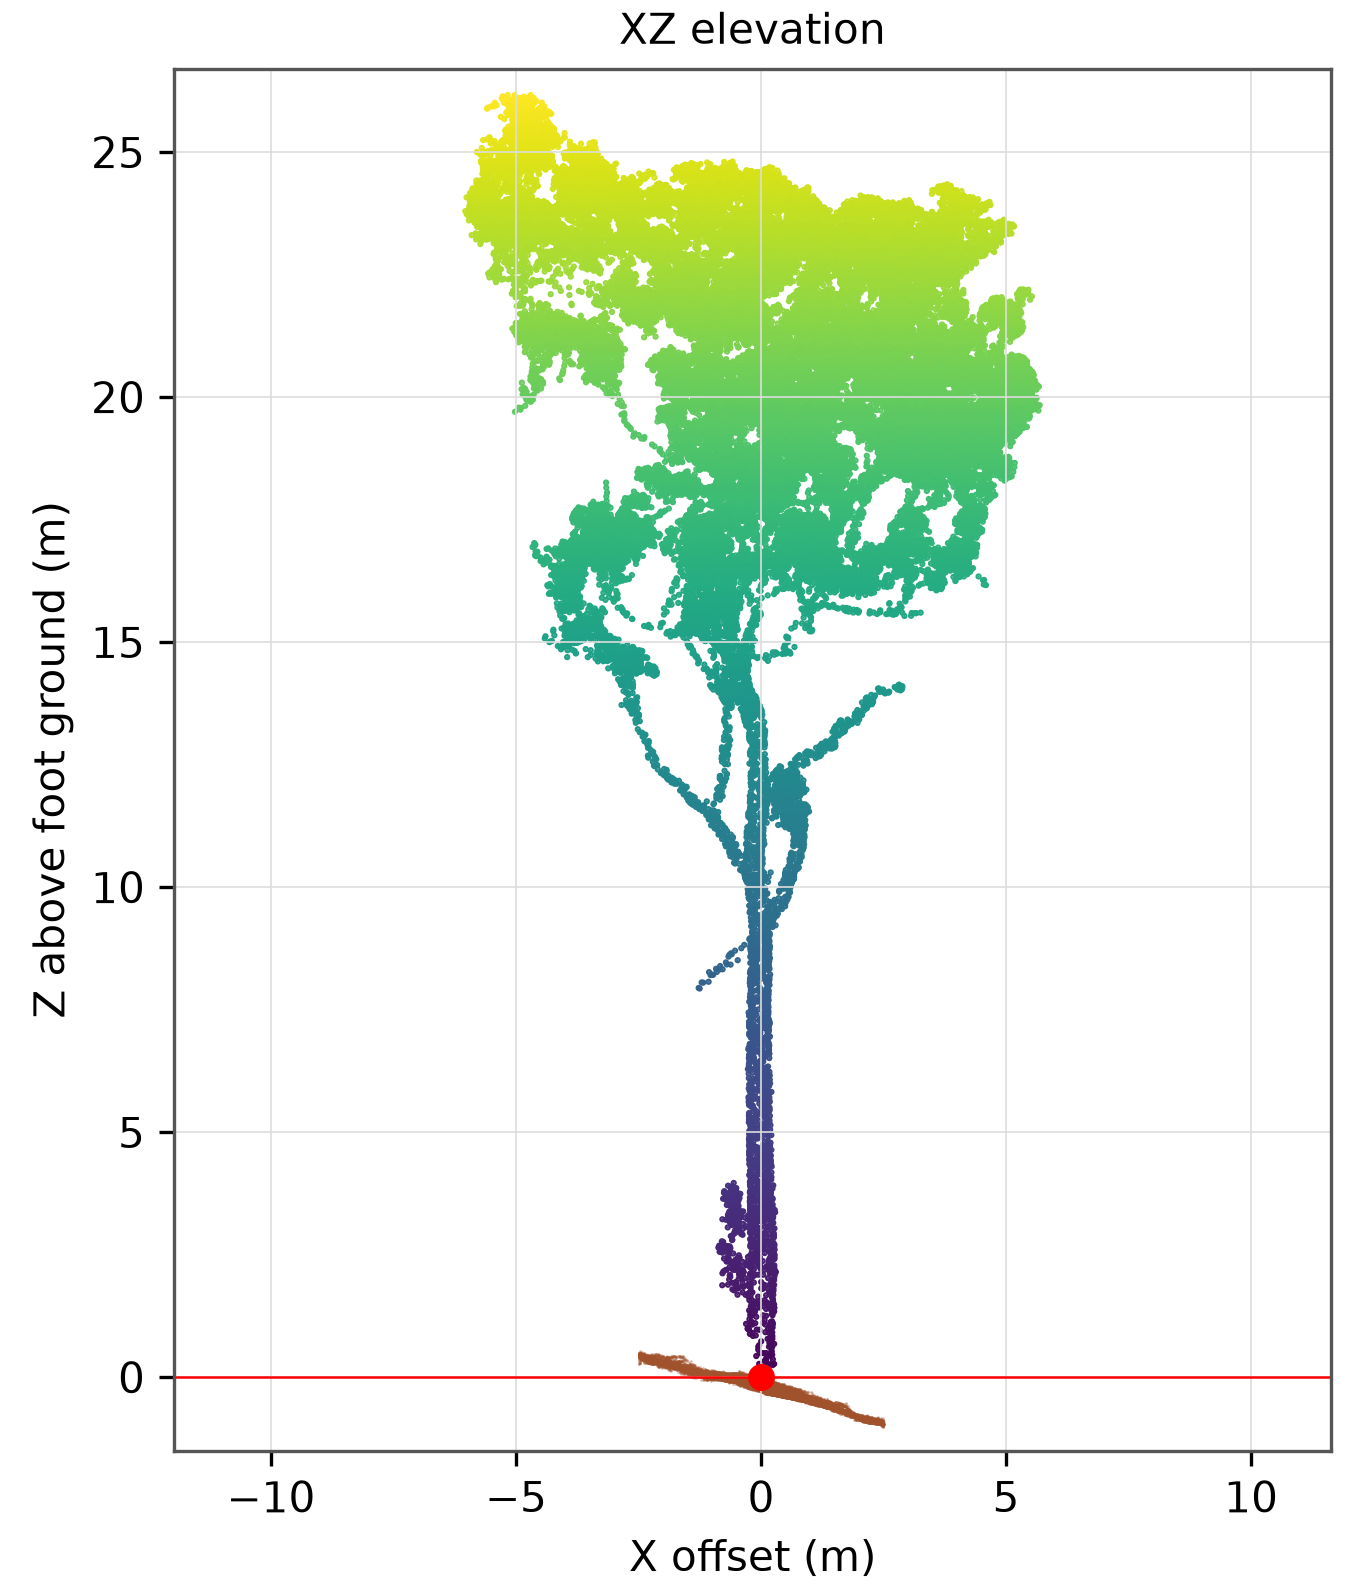
\includegraphics[height=3.7cm]{figures/tree069_xz.png} & 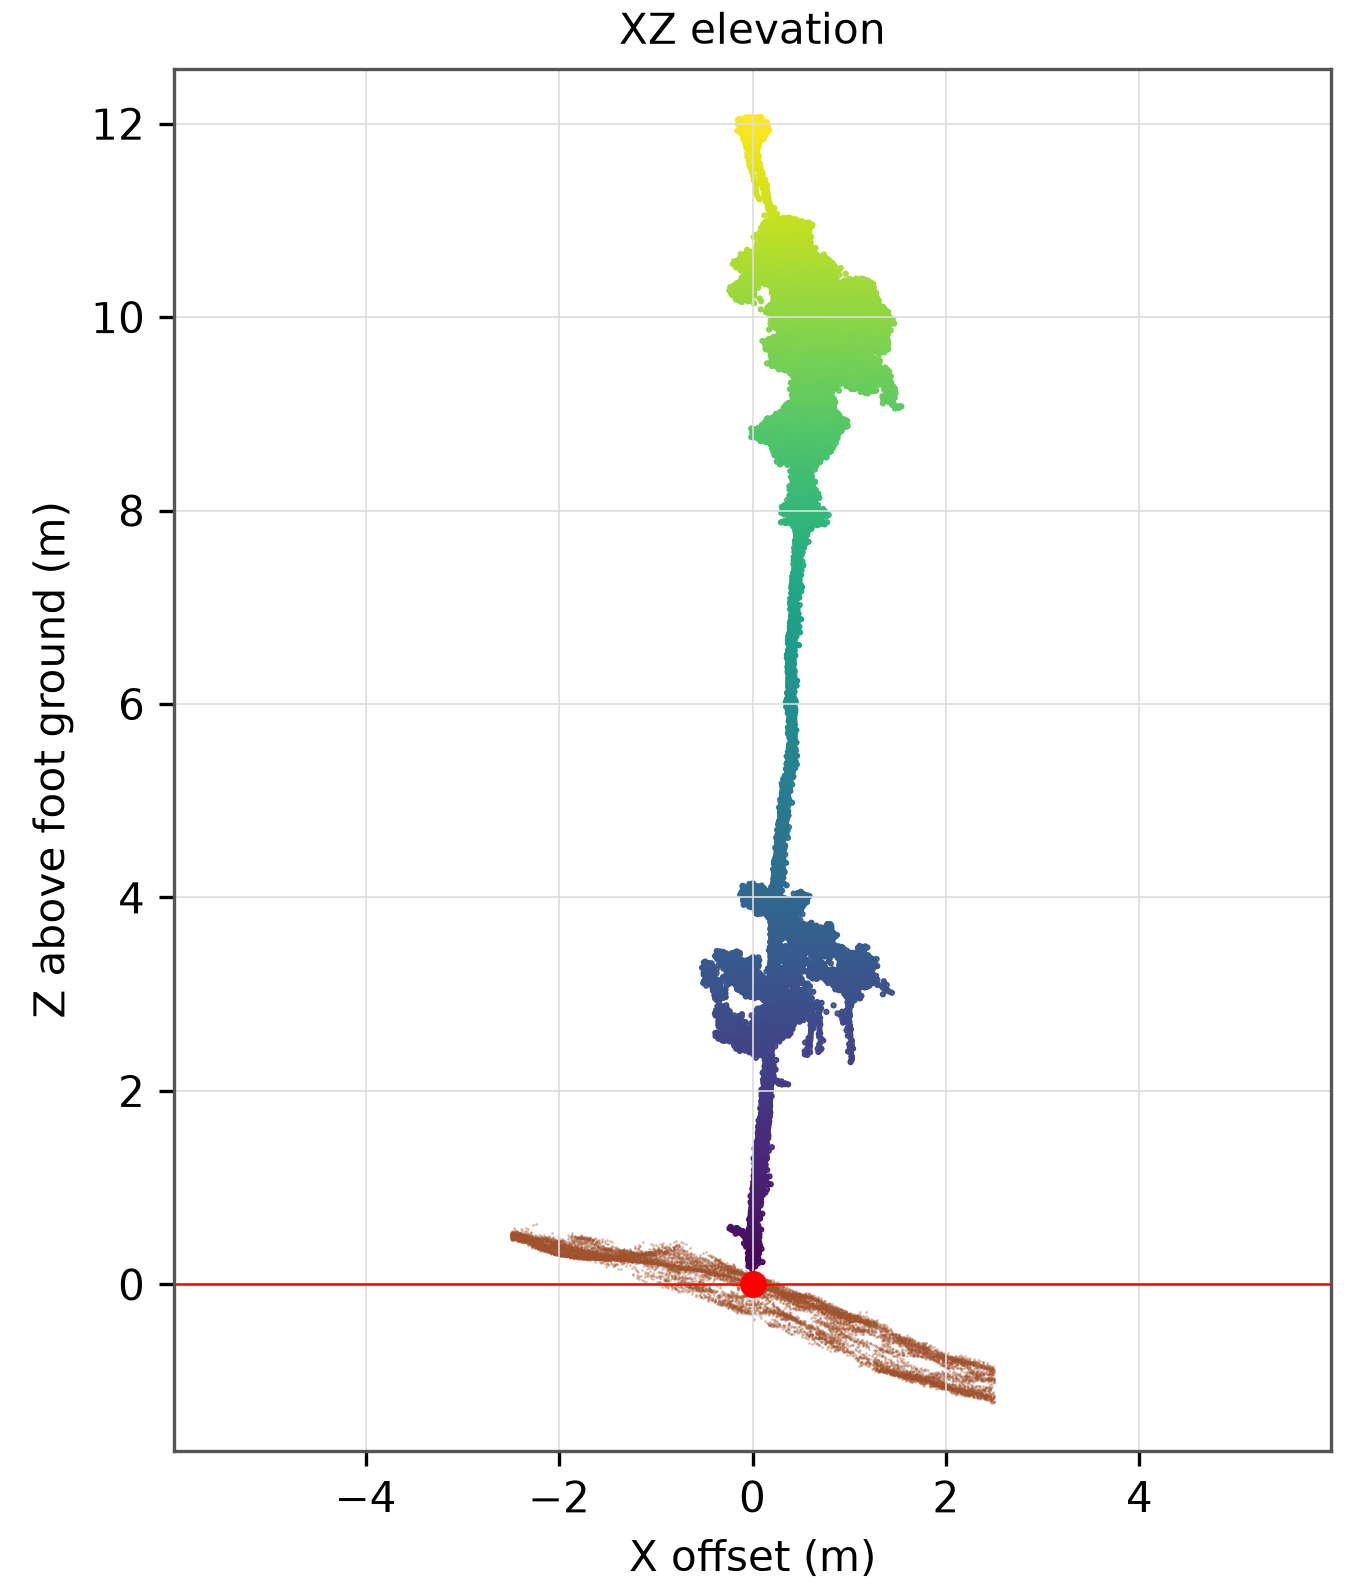
\includegraphics[height=3.7cm]{figures/tree146_xz.png} & 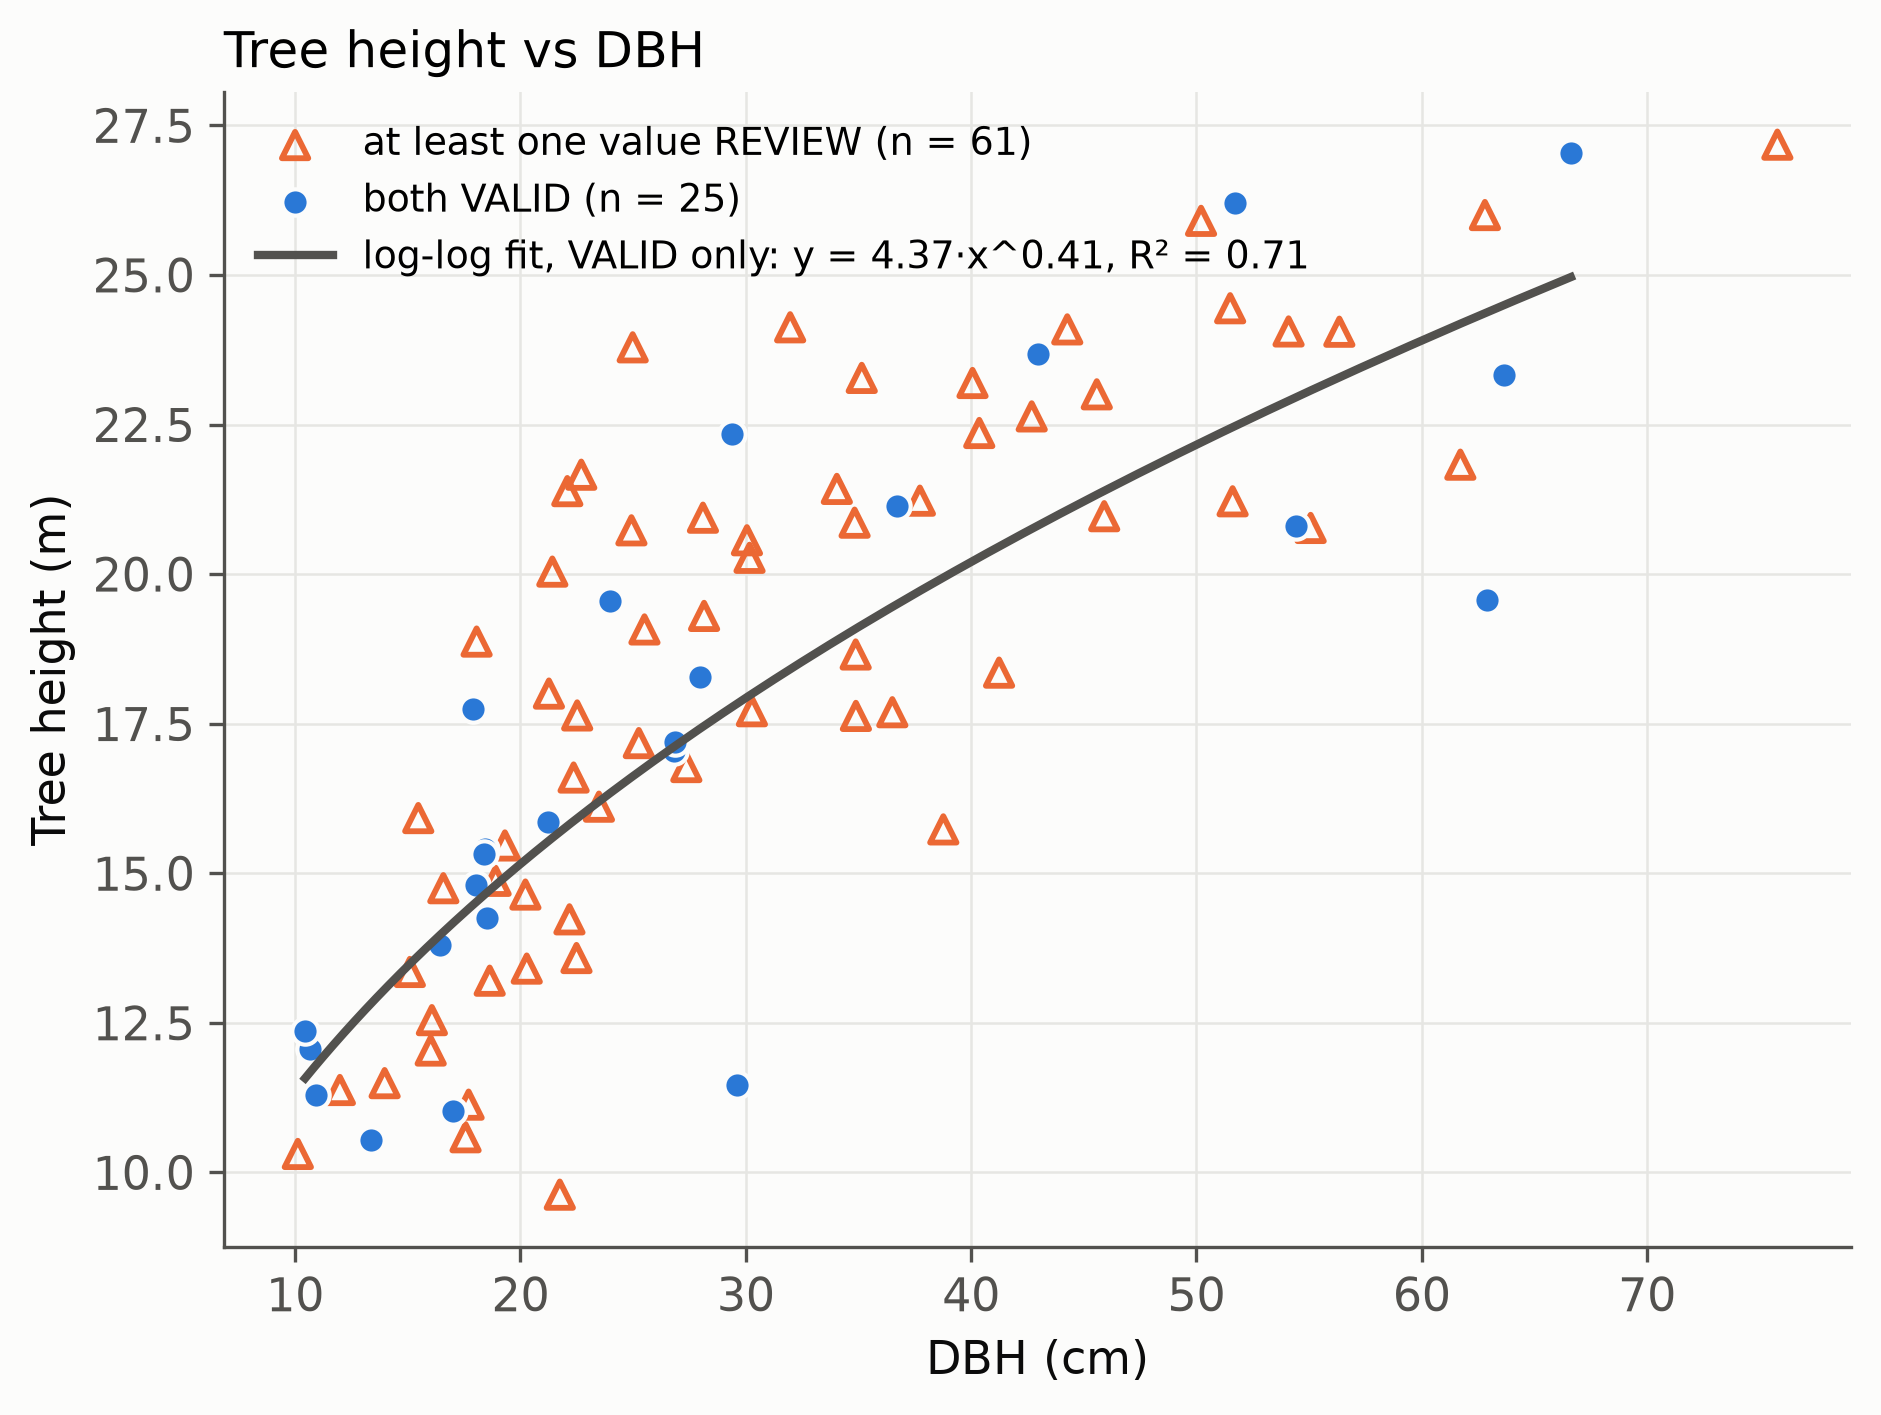
\includegraphics[height=3.7cm]{figures/dbh_vs_height.png}\\[-1pt]
\scriptsize (a) tree\_069 & \scriptsize (b) tree\_146 & \scriptsize (c) Height against DBH
\end{tabular}
\caption{(a, b) Side views of two corrected trees, coloured by height above ground. tree\_069: height 26.2\,m, DBH 51.7\,cm (VALID), crown area 97.6\,m$^2$ (REVIEW). tree\_146: height 12.1\,m, DBH 10.7\,cm (VALID), crown area 1.9\,m$^2$ (REVIEW). (c) Height against DBH for the 86 trees with both values: 25 pairs with both VALID (dots) and 61 with at least one REVIEW value (triangles); the line is a fit to the VALID pairs.}\label{fig:examples}
\end{figure}

\subsection{Field Validation of DBH}\label{sec:res-field}
\emph{The field plot in the scan.} The 30\,m field plot lies inside the TLS crop (Fig.~\ref{fig:match}a). Around the GPS centre, 39 segmented TLS trees have their stem base inside the circle (30 around the map-fitted centre), against 26 live tagged trees in the field; the TLS count includes stems below the field threshold.

\emph{DBH distribution.} Table~\ref{tab:field} compares the TLS trees inside the circle with the 26 live field trees (median 32.5\,cm, largest 107.5\,cm). For the measured DBH, the TLS median is 7.7\% (GPS centre) or 13.8\% (fitted centre) below the field median, and no TLS set differs significantly from the field ($p$ = 0.35--0.91), although with 10--33 trees the test has little power. Adding the estimated DBH lowers the median, because the estimates are mostly for thin stems.
\begin{table}[!tb]
\caption{DBH of TLS trees ($\ge$ 10\,cm) inside the 30\,m field plot against the 26 live field trees (median 32.5\,cm, largest 107.5\,cm; largest TLS 66.6\,cm in every set). Diff.: TLS minus field median, \% of field. GPS: surveyed centre. Fitted: map-fitted centre (sensitivity check).}\label{tab:field}
\centering\footnotesize
\begin{tabular}{@{}llrrrr@{}}
\toprule
Centre & TLS set & $n$ & Median & Diff. & $p$\\
\midrule
GPS & VALID & 16 & 35.8 & $+10.2\%$ & 0.72\\
GPS & Measured & 28 & 30.0 & $-7.7\%$ & 0.62\\
GPS & Meas.\ + est. & 33 & 21.4 & $-34.2\%$ & 0.43\\
Fitted & VALID & 10 & 31.4 & $-3.4\%$ & 0.91\\
Fitted & Measured & 20 & 28.0 & $-13.8\%$ & 0.48\\
Fitted & Meas.\ + est. & 23 & 27.4 & $-15.7\%$ & 0.35\\
\bottomrule
\end{tabular}
\end{table}

\begin{figure}[!tb]
\centering
\begin{tabular}{@{}cc@{}}
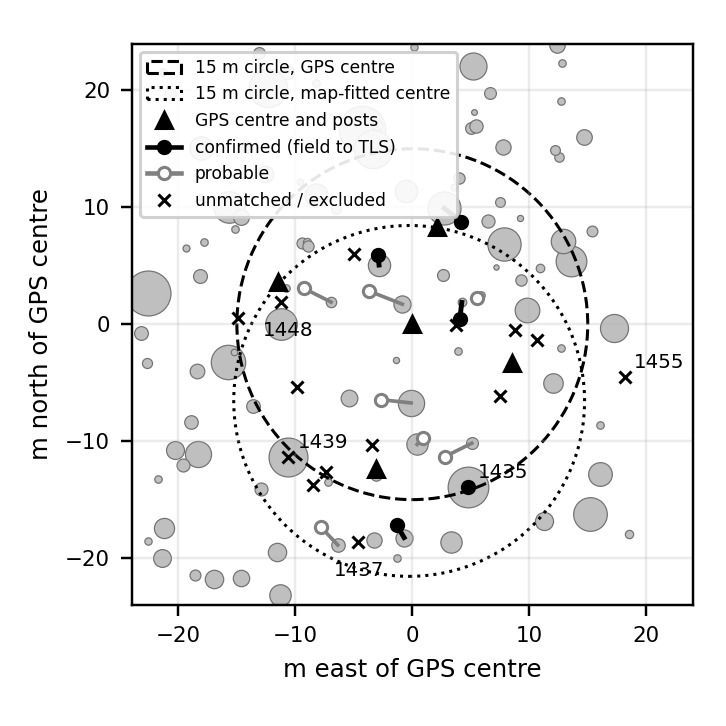
\includegraphics[width=0.48\linewidth]{figures/plot_location_map.png} & 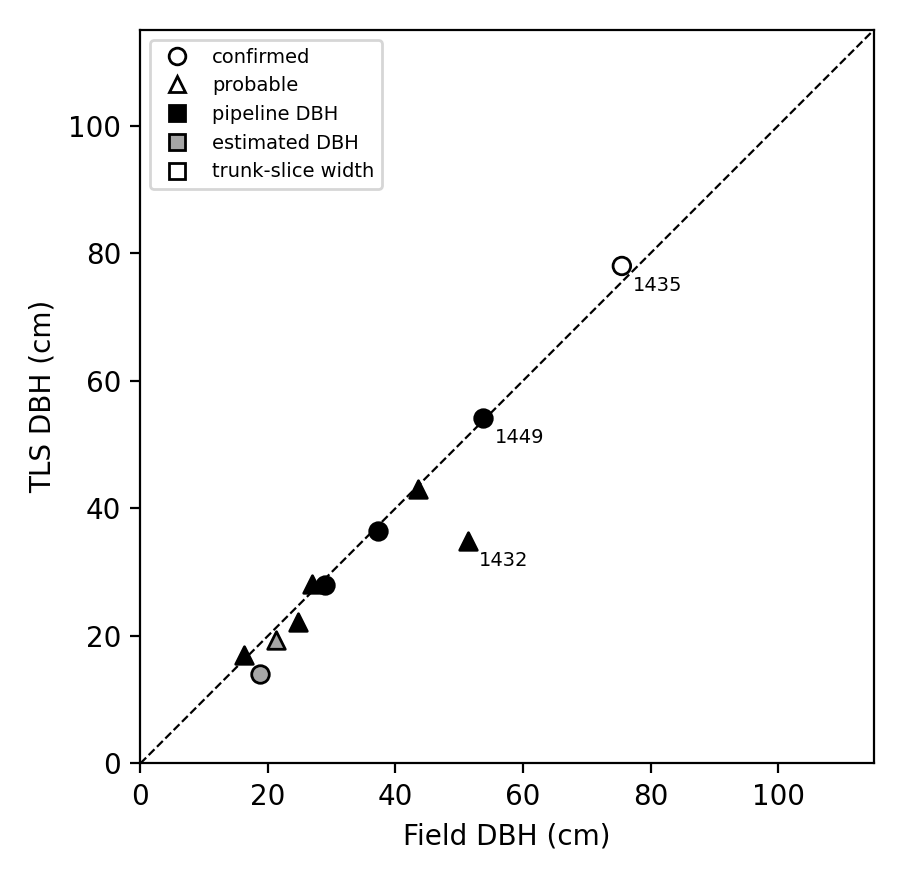
\includegraphics[width=0.48\linewidth]{figures/dbh_matched_scatter.png}\\[-2pt]
\scriptsize (a) Field plot in the TLS crop & \scriptsize (b) Field against TLS DBH
\end{tabular}
\caption{(a) The 30\,m field plot located in the TLS crop (grey: TLS stems, size by DBH), with lines from each tag's predicted map position to its matched TLS stem. (b) DBH of matched trees against the 1:1 line. Confirmed: 1435/103, 1449/102, 1444/089, 1436/091, 1451/106; triangles in (b): probable.}\label{fig:match}
\end{figure}

\emph{Individual trees.} The automatic search failed: placements 13\,m apart matched equally many trees (16 of 26 within 1.5\,m), as did random stem positions (13--16), because the stand is dense and the GPS and map are off by metres. With the two hand-picked anchors, 5 tags are confirmed, 8 probable, 12 unmatched and one excluded (Fig.~\ref{fig:match}). With shuffled DBH values only 1.4 tags were confirmed on average (5 or more in 0.7\% of runs), so the identification is far better than chance. For the 5 confirmed trees, TLS DBH differs from field DBH by $-$0.7\,cm on average (RMSE 2.4\,cm; 4 trees with pipeline DBH: $-$2.6 and 4.5\,cm). 1451/tree\_106 is confirmed on an estimated DBH ($-$25\%). This is a lower bound, because a confirmed pair must agree within 25\%. Including the probable pairs (12 with DBH) gives $-$4.1\,cm and RMSE 9.2\,cm (23\%), driven by 1439/tree\_074 ($-$29\%) and 1432/tree\_098 ($-$32\%), where a wrong pairing and a TLS error cannot be told apart.

\emph{The largest trees.} The pipeline's largest DBH inside either circle is 66.6\,cm, while five field trees are 74.5--107.5\,cm. Matching explains part of this gap. 1435 (75.5\,cm) is tree\_103, an oval trunk of 96\,$\times$\,64\,cm whose circle fit (66.6\,cm) is too low; its area-equivalent width is 78\,cm. 1448 (83\,cm) lies on tree\_079, two intertwined trees (about 80 and 69\,cm) that segmentation could not separate. I checked these trunks visually in CloudCompare and verified the widths with AI-assisted slice fits; on 17 clean, round trunks such slices agree with the pipeline (RMSE 0.9\,cm). 1439 (90\,cm) is probably tree\_074, measured at 63.6\,cm; refits at nine heights gave 55--77\,cm, so the fitting method does not explain the gap. 1437 (107.5\,cm) was not found: the only large live trunk nearby is tree\_163 (about 85\,cm, leaning 63\textdegree), 4--5\,m from the predicted position. 1455 (74.5\,cm) falls at the crop's eastern edge in dense clutter. So the gap has several causes: measurement failure on an oval trunk, a segmentation error that merged two trunks, one large unexplained difference (1439), and two trees that could not be identified.
%======================================================================
\section{Discussion}\label{sec:discussion}

\subsubsection{Answers to the Research Questions.}
\emph{RQ1:} 86 of 163 trees were unchanged, and most correction moved points between trees. \emph{RQ2:} about 106 hours by my own per-tree estimate, 37\% of it on the 30 most complex trees, which were also the hardest to measure; intertwined stems were the hardest task. \emph{RQ3:} height exists for all trees but meets every criterion for 73; DBH for 42 and all four main values for only 16 (Table~\ref{tab:results}). \emph{RQ4:} inside the field plot the TLS DBH distribution is not distinguishable from the field one, and for the 5 confidently matched trees TLS and field DBH agree within a few centimetres; with the probable matches the RMSE is 9.2\,cm.

\subsubsection{Segmentation, Measurement Success and Measurement Accuracy.}
\emph{Segmentation accuracy:} the automatic result could not be used directly: 36.8\% of points were unassigned, and correction moved or removed millions more while the tree count hardly changed. The before/after scores measure change, not accuracy, because there is no independent segmentation reference. \emph{Measurement success:} even after careful correction, only 73 heights, 42 diameters and 16 complete trees meet all quality criteria, and re-checking the flags found stray points that had made four heights 4.0--9.5\,m too tall. A well-segmented tree is necessary but not sufficient for usable traits; I see this as a main result, not only a limitation. \emph{Measurement accuracy:} only DBH has an independent reference. It agrees at plot level and for 5 matched trees, but the matched sample is small and selected partly on agreement, and the largest disagreements involve the largest trees. The internal checks (height--DBH relation, re-implementation, hidden-stem test, trunk slices) show that values are consistent and the procedure repeatable, not that they are correct. VALID trees are also not a random sample, so their medians should not be read as plot averages.

\subsubsection{Why So Many Values Need Review.}
DBH is missing where no stem axis was found (21 trees) or no fit was good enough (55). My analyses do not separate the causes, so the following are hypotheses. Low point density may contribute (14 of the 55 failed fits had fewer than ten points in the slice), as may occlusion, stem shape (forks, leaning or oval trunks such as tree\_163, 079 and 103) and segmentation errors near 1.3\,m~\cite{calders2020,cushman2026}. Refitting DBH on the full-resolution crop (234 million points), which is kept, would test whether thinning contributed to the failures. Height REVIEW labels mostly mean uncertain ground at the stem base or a crown cut by the crop edge, and ground-based TLS may miss the very top~\cite{calders2020,cushman2026}.

\subsubsection{Limitations.}
All 163 trees are accepted as the final set on the visual judgement of two people (Erick Calderon-Morales and me), not by a numerical check; tree\_079 and 8 trees with poor source data stay flagged. The plot location rests on handheld GPS with errors of several metres, the tree matches rest on an approximate map and two anchors, and the survey was 13 months before the scan. Effort is a per-tree estimate made after the work, not a timed log, and error types were not recorded, and some processing settings were not recorded. The study covers one 0.32\,ha crop, and 40 DBH values are estimates checked only against other fits.

%======================================================================
\section{Conclusion and Future Work}\label{sec:conclusion}
I applied a semi-automated workflow to plot WSF\_ML2A: a 0.32\,ha crop was segmented automatically into 162 trees, corrected by hand into 163, and measured with ITSMe under predefined quality criteria. Two lessons stand out. Near-equal tree counts before and after correction hid substantial splitting, merging and reassignment of points, and successful segmentation did not ensure usable measurements: only 16 trees meet every criterion. Inside the located 30\,m field plot the TLS DBH distribution agrees with the field one. Using two hand-picked anchor trees, 5 tagged trees were matched with confidence, and their TLS DBH agrees with the field within a few centimetres. The large-tree gap is explained partly by oval and merged trunks.

Next steps are to confirm the matches and locate 1437 and 1455 in the field (bearing and distance from the centre post; a 12-tree check sheet is ready), to record an accept/reject decision for each tree, and to test whether refitting DBH at full resolution recovers missing values. Biomass needs robust segmentation and structural measurements, so it follows these steps.

\section*{Use of AI}
This statement follows the University's Academic Integrity Policy~\cite{info6003}. I used generative AI assistants (OpenAI Codex and Anthropic Claude) throughout this project. The Python and R scripts (auditing, ITSMe measurement, quality rules, statistics, figures, the RQ1 comparison, crop-edge check, field-plot location, tree matching and trunk slices) were developed interactively with these assistants: I described what was needed, and the code was written, run and revised in conversation with them. The assistants also proposed point recoveries for four trees and crown-base options, from which I chose, developed the DBH fallbacks and height and crown-volume refinements, double-checked my anchor-trunk widths and spacing with geometric fits, at my request, and suggested edits to this report, which I reviewed before applying. I performed the manual segmentation in CloudCompare myself, inspected and verified the anchor trees, made the editing, crown-base and anchor decisions, decided what to report, and checked the report's numbers against the results.

\begin{thebibliography}{99}\setlength{\itemsep}{0pt}
\bibitem{calders2020}
Calders, K., Adams, J., Armston, J., et al.: Terrestrial laser scanning in forest ecology: Expanding the horizon. Remote Sens. Environ. \textbf{251}, 112102 (2020). \href{https://doi.org/10.1016/j.rse.2020.112102}{doi:10.1016/j.rse.2020.112102}

\bibitem{cherlet2026}
Cherlet, W., Dayal, K., Chen, S., et al.: Benchmarking tree instance segmentation of terrestrial laser scanning point clouds. ISPRS J. Photogramm. Remote Sens. \textbf{231}, 230--247 (2026). \href{https://doi.org/10.1016/j.isprsjprs.2025.10.033}{doi:10.1016/j.isprsjprs.2025.10.033}

\bibitem{cushman2026}
Cushman, K.C., Kr\'al, K., Almeyda Zambrano, A.M., et al.: A primer on forest structure measurement with lidar for ecologists. Ecosphere \textbf{17}(8), e70730 (2026). \href{https://doi.org/10.1002/ecs2.70730}{doi:10.1002/ecs2.70730}

\bibitem{lowe2021}
Lowe, T.D., Stepanas, K.: RayCloudTools: A concise interface for analysis and manipulation of ray clouds. IEEE Access \textbf{9}, 79712--79724 (2021). \href{https://doi.org/10.1109/ACCESS.2021.3084954}{doi:10.1109/ACCESS.2021.3084954}

\bibitem{terryn2023}
Terryn, L., Calders, K., \AA{}kerblom, M., et al.: Analysing individual 3D tree structure using the R package ITSMe. Methods Ecol. Evol. \textbf{14}, 231--241 (2023)

\bibitem{meetingnotes}
Meeting notes, INFO6003 tree segmentation project (B.~Choat). Unpublished (3 Aug.\ 2026)

\bibitem{pipeline}
Steps processing pipeline (\nolinkurl{processing_pipeline.pdf}). Unpublished, from my supervisor

\bibitem{treedata}
Blue Mountains plot inventory (\nolinkurl{TreeData.csv}). Unpublished, from my professor

\bibitem{plotdata}
Ecology Hub plot data (\nolinkurl{Ecology_Hub_Plot_Data.xlsx}). Unpublished, from my supervisor

\bibitem{sitemap}
Bullaburra sensor site layout map (20 Feb.\ 2026). Unpublished, from my supervisor

\bibitem{info6003}
Western Sydney University: INFO6003 Postgraduate Research Project, Spring 2026 subject outline, Sects.~1.3 and 3.2.3 (2026)
\end{thebibliography}
\end{document}
